\documentclass{sigchi}

% Use this command to override the default ACM copyright statement (e.g. for preprints). 
% Consult the conference website for the camera-ready copyright statement.


%% EXAMPLE BEGIN -- HOW TO OVERRIDE THE DEFAULT COPYRIGHT STRIP -- (July 22, 2013 - Paul Baumann)
% \toappear{Permission to make digital or hard copies of all or part of this work for personal or classroom use is 	granted without fee provided that copies are not made or distributed for profit or commercial advantage and that copies bear this notice and the full citation on the first page. Copyrights for components of this work owned by others than ACM must be honored. Abstracting with credit is permitted. To copy otherwise, or republish, to post on servers or to redistribute to lists, requires prior specific permission and/or a fee. Request permissions from permissions@acm.org. \\
% {\emph{CHI'14}}, April 26--May 1, 2014, Toronto, Canada. \\
% Copyright \copyright~2014 ACM ISBN/14/04...\$15.00. \\
% DOI string from ACM form confirmation}
%% EXAMPLE END -- HOW TO OVERRIDE THE DEFAULT COPYRIGHT STRIP -- (July 22, 2013 - Paul Baumann)


% Arabic page numbers for submission. 
% Remove this line to eliminate page numbers for the camera ready copy
% \pagenumbering{arabic}


% Load basic packages
\usepackage{balance}  % to better equalize the last page
\usepackage{graphics} % for EPS, load graphicx instead
\usepackage{times}    % comment if you want LaTeX's default font
\usepackage{url}      % llt: nicely formatted URLs

% llt: Define a global style for URLs, rather that the default one
\makeatletter
\def\url@leostyle{%
  \@ifundefined{selectfont}{\def\UrlFont{\sf}}{\def\UrlFont{\small\bf\ttfamily}}}
\makeatother
\urlstyle{leo}


% To make various LaTeX processors do the right thing with page size.
\def\pprw{8.5in}
\def\pprh{11in}
\special{papersize=\pprw,\pprh}
\setlength{\paperwidth}{\pprw}
\setlength{\paperheight}{\pprh}
\setlength{\pdfpagewidth}{\pprw}
\setlength{\pdfpageheight}{\pprh}

% Make sure hyperref comes last of your loaded packages, 
% to give it a fighting chance of not being over-written, 
% since its job is to redefine many LaTeX commands.
\usepackage[pdftex]{hyperref}
\hypersetup{
pdftitle={SIGCHI Conference Proceedings Format},
pdfauthor={LaTeX},
pdfkeywords={SIGCHI, proceedings, archival format},
bookmarksnumbered,
pdfstartview={FitH},
colorlinks,
citecolor=black,
filecolor=black,
linkcolor=black,
urlcolor=black,
breaklinks=true,
}

% create a shortcut to typeset table headings
\newcommand\tabhead[1]{\small\textbf{#1}}


% End of preamble. Here it comes the document.
\begin{document}

\title{From Up or Down: Locating Habitual Reading Region by UnIntrusive Attention Tracking}

\numberofauthors{3}
\author{
  \alignauthor Lei Zhang\\
    \affaddr{Georgia State University}\\
    \affaddr{Atlanta,Georgia,U.S.A}\\
    \email{lzhang14@student.gsu.edu}
  \alignauthor Ying Zhu\\
    \affaddr{Georgia State University}\\
    \affaddr{Atlanta,Georgia,U.S.A}\\
    \email{yzhu@cs.gsu.edu}
}

\maketitle

\begin{abstract}

In this paper, we present our research on detecting habitual reading region 
on the screen when a user is doing his daily online reading. Instead of traditional eye-tracking based solution,
we developed an unintrusive user attention tracking(UUAT) solution. In UUAT, we developed a ReadingClue 
technology,  which helps to pinpoint user reading attention when necessary. At the same time, user reading behavioral data(mouse click and mouse scroll) is
collected in background. With these behavioral data, UUAT calculates a user's preferred reading range. Our experiment
indicates that the accuracy of UUAT attention tracking is as high as 93.2\%.





\end{abstract}

\keywords{
	Attention Tracking; Reading; Mouse movements; Scrolling;
}

\category{H.5.m.}{Information Interfaces and Presentation (e.g. HCI)}{Miscellaneous}

See: \url{http://www.acm.org/about/class/1998/}
for more information and the full list of ACM classifiers
and descriptors. \newline
\textcolor{red}{Optional section to be included in your final version, 
but strongly encouraged. On the submission page only the classifiers’ 
letter-number combination will need to be entered.}

\section{Introduction}

Personal Data Mining\cite{ozzie2011personal}(PDM) has been proposed as a complement to commercial/business data mining, which aims to get useful knowledge to improve business opportunity or products popularity. Unlike the concept of commercial data mining, PDM is proposed for a user’s individual good. In PDM, user behavioral data is collected by a neutral utility. The user can choose third-party tools(local) or service(cloud) to analyze his personal data, aiming to improve individual productivity or quality of life.

 
	As the first step of PDM, Self-Tracking\cite{swan2009emerging} was proposed to log personal data, so that future analysis can be conducted for a user’s good in health. Self-Tracking has been mainly involved in personal physical data, such as, weight, heartbeat, diet and sports. Moreover, the way of logging data has been mainly referred to manual logging, e.g. a user input his weight before going to bed everyday. In this paper, we argue that the reign of personal data is more than physical data and the ways to collect personal data can be extended to an automatic and stealthy way. 


In this research, we consider a user’s daily reading as a source of personal data. An immediate reason is that to understand a user’s daily reading helps to build a user’s personal knowledge demography, let alone “For many self-trackers, the goal is unknown”\cite{wolf2010data}. We do not consider what a user have read as static data, instead, we consider it as dynamic. For example, if a user spend more unit reading time on  paragraph 1 than average, this might indicate that the user might have pondered on the information in paragraph 1 or have reading struggles on paragraph 1. In either case, it might indicate that the user has encountered new knowledge and he takes time to digest this new information. From this point of view, it might be a mileage for personal knowledge acquisition, e.g., today is the day I first come to know the concept of “shale gas”, although I have read the same phrase years ago. To log this type of personal data, it is unlikely to adopt the same user-aware way, a more intelligent and stealthy method is required to obtain personal reading data. 

In this research, we focus on how to collect objective and detailed reading behavioral data, so that the PDM can be conducted on an accurate and correct basis. To be specific, we focus on a user’s daily online reading activity, our goal is to accurately identify what texts a users read that day and to what extent he spent on specific parts of an article. To realize this goal, we developed a browser-based solution to obtain a user’s preferred reading scope on a screen, by analyzing the user’s mouse/keyboard input, we provide details on user’s dwell time on each information piece(currently our granularity is paragraph-based). By doing this, we enable a more extensive PDM applications which we will discuss in future work of this paper. Our contributions are as follows: 1.We developed an almost UnIntrusive User Attention Tracking utility, which helps to get a user’s preferred reading scope in a stealthy way. 2. We developed  a solution to get a users daily reading data which can be used as input for deep personal data mining. 


\section{Related Work}

The idea of quantified self-tracking is well known proposed in \cite{wolf2010data}. In \cite{wolf2010data}, the author advocates collecting individual quantified data. He presents cases where individual data collection helped to solve person-specific problems. For example, Barbier used her personal data to find a way to cure her insomnia\cite{wolf2010data},  Seth Roberts, a Caltech professor, analyzed his personal data and find an optimum diet(flaxseed oil) to improve his math performance\cite{wolf2010data}. In this paper, the author advocates a diversified personal data collection, as long as the data is quantified, albeit you might not know the goal of your data collection immediately. 


Since the current personal data mainly includes personal physical data, such as weight, glucose, heartbeat, sports, food/medication consumption. The pervasive methods of personal data collection are mainly by a user himself, such as the methods adopted by PatientsLikeMe\cite{plm}. 


	Our proposed research is very similar to the work in the field of computer human interaction(HCI). To get a user’s preferred reading scope on a screen, there are mainly two categories of solutions, method of eye-track based and method of user input tracking.  
Although having the advantages of highly goal-revealing and providing more details, eye-tracking\cite{jacob2003eye} methods are also tagged as intrusive and expensive. It is impractical to popularize an eye-tracking based application to a large scale, in fact, the eye-tracking method are mainly applied in the software usability test. 


Compared to eye-tracking method, our proposed research is closer to the method of user input tracking \cite{navalpakkam2012mouse,huang2011no,lagun2011viewser,atterer2007tracking,10}.  The authors of \cite{navalpakkam2012mouse} collected user mouse data, at the same time they collected user’s eye gaze data, they proved that the user mouse data can indicate user behavior, e.g. which part of the screen is more attractive, the user distraction behavior can be detected and the user experience can be predicted by mouse analysis in an accuracy of 80%. The result of this research is highly depend on the eye-gaze data and we argue that the user behavior might be changed once a subject is put into a headset device and knowing he might be taped in a video. The research of \cite{atterer2007tracking} are conducted in a goal of software usability test. They collect user data in an implicit(stealthy) way, which is more objective. The collected data is very detail focused, which might be used to construct a “playback” for a tester’s tryout. The downside of this research is that it needs to log every interaction between a user and a web component(not a web page, but each HTML components in that webpage),  e.g. how long does it take the tester to first click on a specific radio button on a page. This makes it a difficult knowledge in the context of web2.0. So a further research\cite{atterer2006knowing} is conducted on how to log user interaction with Ajax-based web components. Since the research goal is to evaluate a software usability, the work in \cite{atterer2007tracking,atterer2006knowing} collects data in a raw and  particular way. Furthermore, extra server-side support is needed to conduct the data collection, making it less scalable. The research of \cite{huang2011no} are conducted for evaluation of search engine result pages. Both of them collect data for the goal to discover which search engine result item is more attractive to a user. In \cite{huang2011no}, the author proposed a “viewport” technology, which blurs all the other result items except one item, so that the user can put his attention on result item. In this way, the user is forced to locate his reading range to where the unblurred item is.  In \cite{lagun2011viewser}, the author also tries to make use of mouse data, but they are more interested in the mouse trajectory instead of the mouse click, since the mouse is more often to move in the screen than a mouse is clicked, but the mouse move does not always trigger an event that can be logged. With the comparison of eye-gaze data, they disclose that the mouse trajectory can be used to infer a user’s interest on the search engine result items. 
By literature review we distinguish our research from existing works as follows: the data collection in our research is designed to be more scalable, so our data collection method can be tagged as "unintrusive", unlike the eye-gaze technology adopted in \cite{navalpakkam2012mouse,lagun2011viewser}. Meanwhile our goal is personal data collection instead of usability test, we proposed a new CHI technology to accurately infer user’s preferred reading range on the screen, so that we can collect high quality data that can describe a user’s daily reading behavior objectively. 


\section{The Assumption, Model }
\subsection{Model}

The previous research on user attention tracking \cite{buscher2010eye} have disclosed some facts when a user is doing daily reading on 
articles or document papers. Vertically, in most of the time, the reading progresses towards the end of the screen  in a line-by-line manner. 
However, the reading does not start from the first line on the screen until the last line of the screen. Generally, a user has a preferred reading region on screen,
as indicated in figure \ref{fig:read_region}. A preferred reading region can be identified by two parameters $\Delta_0$ and $w$. $\Delta_0$  indicates the 
offset from the head of the screen and $w$ indicates the vertical width of the whole region. If a user wants to read the contents outside the region,
a scroll action is expected. In this research, we take aforementioned assumption and model the user attention range as displayed in figure \ref{fig:read_region}. 



\begin{figure}[!h]
\centering
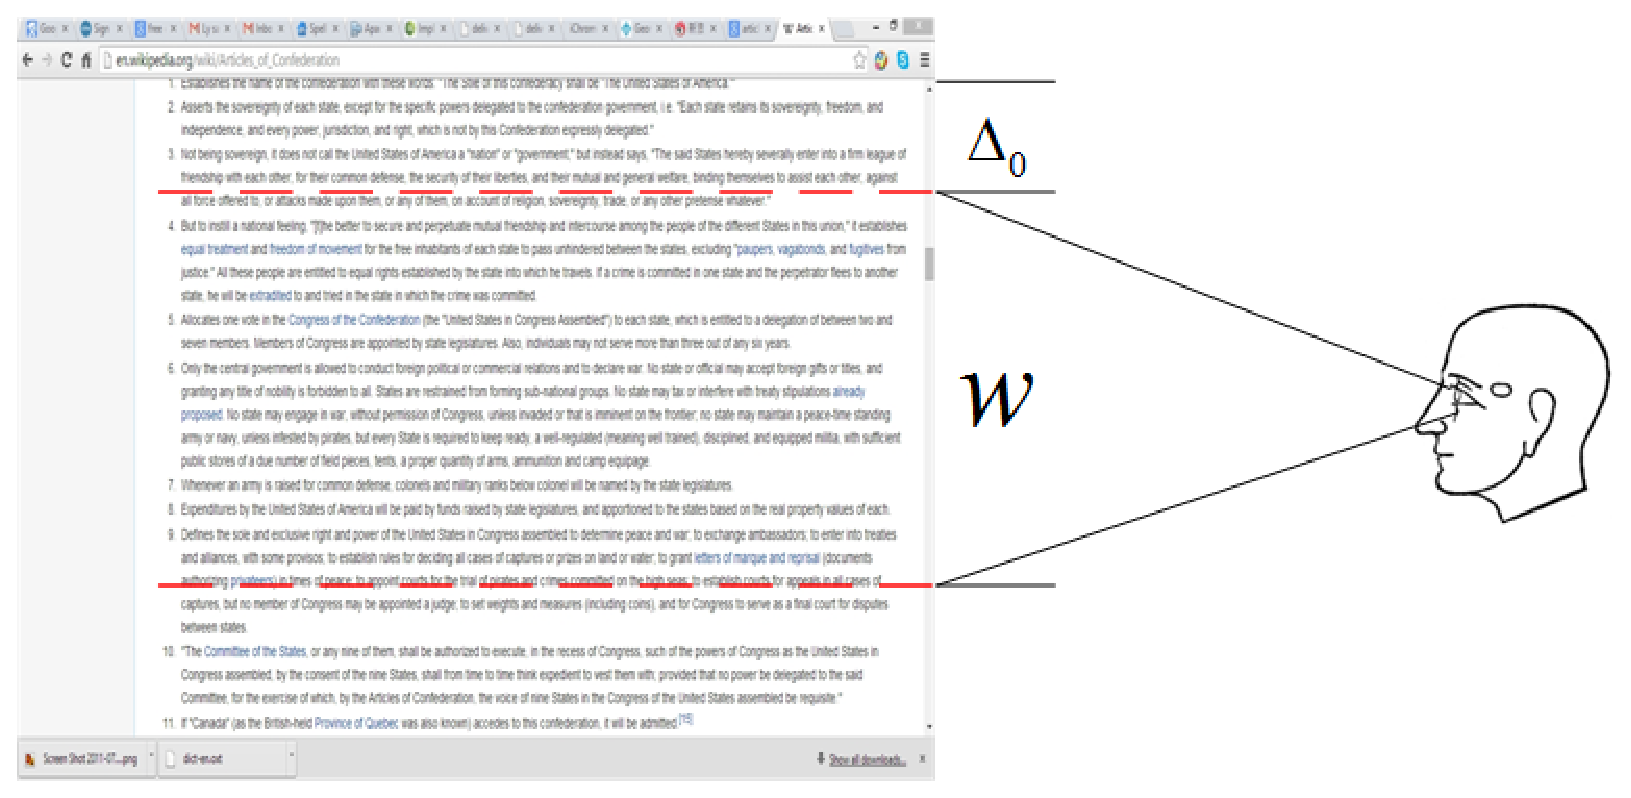
\includegraphics[width=1.0\columnwidth]{pictures/preferred_reigon}
\caption{The preferred reading region on the screen}
\label{fig:read_region}
\end{figure}



Taking this model into consideration, our next  research question is: 
What behavioral data should be collected and analyzed?


Eye tracking data can be easily mentioned to answer the question, especially when a "visual" reading range is 
the goal. However, we argue that the eye tracking data has twofold major drawbacks: 1. The eye tracking collection 
requires extra hardware, which means the eye tracking  based solution  is not scalable and very costly. 2. What is even worse, 
eye tracking is "intrusive". A subject person is aware that he is wearing a headset device and he is under a camera coverage, 
his behavior is very likely to be different from how he behaves when he is doing reading alone. For these two reasons, we 
can not use eye tracking data. To meet the requirement of unintrusive but objective, the only option left is the user interaction data 
collected when the reading is ongoing.  In the next section we will discuss how to 
collect and analyze user interaction data to get the user preferred region.  


\subsection{Calculating User Preferred Region by Interaction Data}

When a user is doing daily reading,  since the keyboard input rarely happens 
during the reading process,  we are more interested in the mouse-generated data. 
There are two categories of mouse-generated data, mouse click and scroll.  We consider the mouse-generated data to be 
informational  behavioral data. To be specific, a  mouse click indicates the position of user's reading attention at that time instant, 
a page scroll indicates how much contents has been moved out of reading region. Our next question is how to infer 
preferred reading region by collected mouse-generated data. 


\begin{figure*}[t]
\centering
\includegraphics[width=1.5\columnwidth]{pictures/scroll}
\caption{Reading of a long article in a browser}
\label{fig:scroll}
\end{figure*}

Now we examine a typical online reading event, during which a user finishes reading of a whole article. We suppose 
 the article is relatively long, which requires many scroll action. The whole reading process can be illustrated by figure \ref{fig:scroll}


In figure \ref{fig:scroll}, a user conducts a scroll action when he finishes reading contents of current reading region. 
At $i$th scroll action, a $\Delta_i$ of page height will be moved out of region. So when the article reading is finished, 
we have equation (\ref{eq:1}). In equation (\ref{eq:1}) , $\Delta_0$ and $w$ are defined in figure 
\ref{fig:read_region}. Ideally, equation (\ref{eq:2}) should hold and the parameter $w$ can be 
calculated in equation (\ref{eq:3}). In practice, it is unlikely for equation (\ref{eq:2}) to strictly hold,
however, equation (\ref{eq:1}) can still be applied. 

\begin{equation} \label{eq:1}
	H = \sum\limits_{i = 1}^n {{\Delta _i} + {\Delta _0} + w} 
\end{equation}

\begin{equation} \label{eq:2}
	{\Delta _1} = {\Delta _2} = ... = {\Delta _n} = w
\end{equation}

\begin{equation} \label{eq:3}
	w = \frac{{\sum\limits_{i = 1}^n {{\Delta _i}} }}{n}
\end{equation}


Now that equation (\ref{eq:2}) does not always hold, if the variance of $\Delta_i$ is relatively large(actually it is),
we need to consider the question how to infer user reading  region on each single scroll. Figure \ref{fig:single_click}
displays a the events happened during  reading between two scroll actions. Here red dots are collected mouse click data with
the position on the corresponding place on the screen. Since we take the assumptions that the reading process progresses 
line by line and the mouse click is an indication of instantaneous user attention, we can calculate a minimum reading range after $i_th$ scroll action, 
$w_i^{\min }$, which can be identified by highest click and lowest click(as indicated in figure  \ref{fig:single_click}). 


\begin{figure}[!h]
\centering
\includegraphics[width=0.7\columnwidth]{pictures/single_click}
\caption{Mouse click and reading region}
\label{fig:single_click}
\end{figure}

However, $w_i^{\min }$ is a minimum approximate of $w_i$, we can have a more accurate approximate if we take the neighboring 
scroll actions into consideration. In figure \ref{fig:neighbor_scroll}, we put the click data both before $i$th scroll(purple dots) and after $i+1$th(yellow dots).
We can see there is a gap between two neighbor minimum approximates. So we can have a moderate estimate of $w_i$:


\begin{equation} \label{eq:4}
{w_i} = w_i^{\min } + ({g_1} + {g_2})/2
\end{equation}
 

\begin{figure}[!h]
\centering
\includegraphics[width=0.9\columnwidth]{pictures/neighbor-scroll}
\caption{Mouse click and reading region}
\label{fig:neighbor_scroll}
\end{figure}


\bibliographystyle{acm-sigchi}
\bibliography{sample}
\end{document}
